\documentclass[a4paper, 12pt]{report}
\usepackage{cmap}
\usepackage{amssymb}
\usepackage{amsmath}
\usepackage{graphicx}
\usepackage{amsthm}
\usepackage{upgreek}
\usepackage{setspace}
\usepackage{color}
\usepackage{moreverb}
\usepackage[T2A]{fontenc}
\usepackage[utf8]{inputenc}
\usepackage[normalem]{ulem}
\usepackage{mathtext} % русские буквы в формулах
\usepackage[left=2cm,right=2cm, top=2cm,bottom=2cm,bindingoffset=0cm]{geometry}
\usepackage[english,russian]{babel}
\usepackage[unicode]{hyperref}
\newenvironment{Proof} % имя окружения
{\par\noindent{$\blacklozenge$}} % команды для \begin
{\hfill$\scriptstyle\boxtimes$}
\newcommand{\Rm}{\mathbb{R}}
\newcommand{\Cm}{\mathbb{C}}
\newcommand{\Z}{\mathbb{Z}}
\newcommand{\I}{\mathbb{I}}
\newcommand{\N}{\mathbb{N}}
\newcommand{\rank}{\operatorname{rank}}
\newcommand{\Ra}{\Rightarrow}
\newcommand{\ra}{\rightarrow}
\newcommand{\FI}{\Phi}
\newcommand{\Sp}{\text{Sp}}
\renewcommand{\leq}{\leqslant}
\renewcommand{\geq}{\geqslant}
\renewcommand{\alpha}{\upalpha}
\renewcommand{\beta}{\upbeta}
\renewcommand{\gamma}{\upgamma}
\renewcommand{\delta}{\updelta}
\renewcommand{\varphi}{\upvarphi}
\renewcommand{\phi}{\upvarphi}
\renewcommand{\tau}{\uptau}
\renewcommand{\lambda}{\uplambda}
\renewcommand{\psi}{\uppsi}
\renewcommand{\mu}{\upmu}
\renewcommand{\omega}{\upomega}
\renewcommand{\d}{\partial}
\renewcommand{\xi}{\upxi}
\renewcommand{\epsilon}{\upvarepsilon}
\newcommand{\intx}{\int\limits_{x_0}^x}
\newcommand\Norm[1]{\left\| #1 \right\|}
\newcommand{\sumk}{\sum\limits_{k=0}^\infty}
\newcommand{\sumi}{\sum\limits_{i=0}^\infty}
\newtheorem*{theorem}{Теорема}
\newtheorem*{cor}{Следствие}
\newtheorem*{lem}{Лемма}
\begin{document}
	% Оформление титульного листа
	\begin{titlepage}
		\begin{center}
			\textsc{МИНИСТЕРСТВО ОБРАЗОВАНИЯ РЕСПУБЛИКИ БЕЛАРУСЬ БЕЛОРУССКИЙ ГОСУДАРСТВЕННЫЙ УНИВЕРСИТЕТ
				\\[5mm]
				ФАКУЛЬТЕТ ПРИКЛАДНОЙ МАТЕМАТИКИ И ИНФОРМАТИКИ\\[2mm]
				Кафедра компьютерных технологий и систем
			}
			
			\vfill
			
			\textbf{Отчет по лабораторной работе №1\\
				«Решение задач Коши и Гурса для уравнений в частных
				производных второго порядка при помощи Wolfram
				Mathematica»\\
				Вариант 2
				\\[26mm]
			}
		\end{center}
		
		\hfill
		\begin{minipage}{.5\textwidth}
			\begin{flushright}
				Бовта Тимофея Анатольевича\\
				студента 3 курса\\
				специальности «прикладная математика»\\[5mm]
				
				Преподаватель:\\[2mm] 
				И. С. Козловская\\
			\end{flushright}
		\end{minipage}%
		\vfill
		\begin{center}
			Минск, 2024\ г.
		\end{center}
	\end{titlepage}
	\newpage
	\section*{Постановка задачи.}
	Дана задача $$\begin{cases}
		u_{xy} + xu_y =y,\\
		u|_{x=0} = 1,\\
		u|_{y=0} = x+1.
	\end{cases}$$
	\begin{itemize}
		\item найти решение данной задачи Коши или Гурса;
		\item проверить полученное решение путем подстановки в уравнение и
		условия задачи;
		\item построить график поверхности $z = u(x,y)$, где $u$ -- решение задачи.
	\end{itemize}
	\section*{Решение задачи.}
	Сперва зададим задачу и граничные условия в Wolfram Mathematica:
	\begin{listingcont}
In[1]:= eq = Derivative[1, 1][u][x, y] + x*Derivative[0, 1][u][x, y] == y;
	cc = {u[0, y] == 1, u[x, 0] == x + 1}

Out[2]= {u[0, y] == 1, u[x, 0] == 1 + x}\end{listingcont}
Определимся с тем, что перед нами поставлена задача Гурса. Так как исходное уравнение является уравнением гиперболического типа, а условия -- краевыми (в случае задачи Коши условия являются начальными).\\\\
Проверим выполнение условий согласования, то есть оба условия должны выполняться на множестве, где для всех $x$ и $y$ выполняется $$u(0, y) = u (x, 0).$$
	\begin{listingcont}
In[3]:= intersect = Solve[{x == 0, y == 0}, {x, y}]

Out[3]= {{x -> 0, y -> 0}}

In[4]:= cc[[1, 2]] == cc[[2, 2]] /. intersect[[1]]

Out[4]= True\end{listingcont}
Таким образом, условия поставленной задачи Гурса согласованы. \\\\
Вернемся к рассмотрению исходного уравнения в поставленной задаче. Можно заметить, что данное уравнение уже является уравнением гиперболического типа в каноническом виде. Более того мы можем найти его общее решение, применив замену $$\dfrac{\partial u}{\partial y} = v(x,y).$$
Тогда при подстановке данной замены исходное уравнение примет вид $$\dfrac{\partial v}{\partial x} + xv = y.$$
Полученное уравнение является линейным обыкновенным дифференциальным уравнением первого порядка (ЛОДУ-1). Мы можем найти его решение с помощью Wolfram Mathematica:
\begin{listingcont}
In[5]:= vsol = DSolve[Derivative[1, 0][v][x, y] + x*v[x, y] == y, v, {x, y}]
\end{listingcont}
$$
	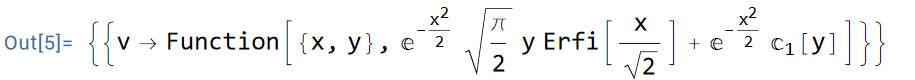
\includegraphics[scale=0.5]{img1}
$$
Решение данного уравнения мы также можем найти и самостоятельно. Для этого необходимо домножить данное уравнение на $e^{\int_0^x x dx}$, свернуть левую часть уравнения как производную произведения, а затем проинтегрировать обе части уравнения по $x$. В итоге получим $$v(x,y) = e^{-\frac{x^2}{2}}C_1(y) + ye^{-\frac{x^2}{2}} \underbrace{\int\limits_0^x e^{\frac{t^2}{2}}dt}_{\sqrt{\frac\pi2} erfi\left(\frac {x}{\sqrt2}\right)}.$$
Сделаем обратную замену и получим простейшее обыкновенное дифференциальное уравнение первого порядка
$$\dfrac{\partial u}{\partial y} = e^{-\frac{x^2}{2}}C_1(y) + ye^{-\frac{x^2}{2}} \int\limits_0^x e^{\frac{\xi^2}{2}}d\xi.$$
Данное уравнение можно решить, проинтегрировав обе части уравнения по $y$. В итоге мы и получим общее решение исходного уравнения в частных производных. Сперва проинтегрируем это уравнение с помощью Wolfram Mathematica:
\begin{listingcont}
In[6]:= usol = DSolve[Derivative[0, 1][u][x, y] == v[x, y] /. 
vsol[[1]], u, {x, y}]
\end{listingcont}
$$
	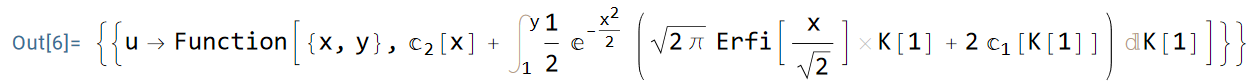
\includegraphics[scale=0.5]{img2}
$$
Полученный вид общего решения является слишком сложным для дальнейшей работы. Проинтегрируем уравнение вручную и проведем некоторые преобразования для упрощения вида общего решения:
$$u(x,y) = e^{-\frac{x^2}{2}}\int\limits_0^yC_1(\eta)d\eta + \int\limits_0^y\eta e^{-\frac{x^2}{2}} \int\limits_0^x e^{\frac{\xi^2}{2}}d\xi d\eta + C_2(x).$$
Сделаем замену $$\int\limits_0^yC_1(\eta)d\eta = C_1(y),$$
где функция $C_1(y)$ справа, вообще говоря, отлична от подынтегральной функции слева, но для упрощения записи будем использовать такое обозначение, так как оно не повлияет на дальнейшее решение. Тогда, если переставим местами интегралы, имеем
$$u(x,y) = e^{-\frac{x^2}{2}}C_1(y) + e^{-\frac{x^2}{2}}\int\limits_0^y\eta d\eta  \int\limits_0^x e^{\frac{\xi^2}{2}}d\xi + C_2(x).$$
Интеграл по $\eta$ мы можем вычислить. В итоге имеем более простую запись общего решения исходной задачи
$$u(x,y) = e^{-\frac{x^2}{2}}C_1(y) + \dfrac{y^2}{2}e^{-\frac{x^2}{2}}\int\limits_0^x e^{\frac{\xi^2}{2}}d\xi + C_2(x).$$
Но нас интересует частное решение поставленной задачи. Его мы можем получить, подставляя заданные условия в полученное общее решение.\\\\
В Wolfram Mathematica переопределим замену usol согласно сделанным преобразованиям. После чего подставим в эту функцию условия на характеристиках из исходной задачи. При этом используем также функцию «Activate», раскрывающую так называемые неактивные интегралы. В итоге имеем
\begin{listingcont}
In[7]:= usol = 
	u -> Function[{x, y}, E^(-x^2/2)*C[1][y] + C[2][x] +
		y^2/2*E^(-x^2/2)*Inactive[Integrate][E^(t^2/2), {t, 0, x}]];
newcc = Activate[cc /. usol]
\end{listingcont}
$$
	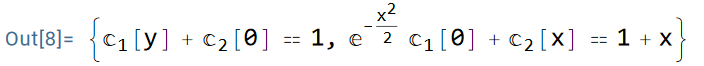
\includegraphics[scale=0.5]{img3}
$$
То есть мы получили систему уравнений относительно функций $C_1(y)$ и $C_2(x)$
$$\begin{cases}
C_1(y) + C_2(0) = 1,\\
e^{-\frac{x^2}{2}} C_1(0) + C_2(x) = 1+x.
\end{cases}$$
Решив ее, мы найдем значения для $C_1(y)$ и $C_2(x)$, подставляя которые в общее решение исходного уравнения, мы найдем вид частного решения поставленной задачи Гурса.\\\\
Из первого уравнения системы выразим $C_1(y)$, причем заменив $C_2(0) = t.$ Имеем 
\begin{listingcont}
In[9]:= c1sol = RSolve[newcc[[1]] /. C[2][0] -> t, C[1], y]
\end{listingcont}
$$
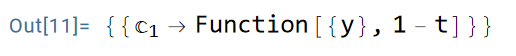
\includegraphics[scale=0.5]{img4}
$$
Получившуюся функцию подставим во второе уравнение системы:
\begin{listingcont}
In[12]:= newcc[[2]] /. c1sol[[1]] /. C[2][0] -> t
\end{listingcont}
$$
	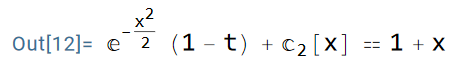
\includegraphics[scale=0.5]{img5}
$$
Найдем функцию $C_2(x)$:
\begin{listingcont}
In[13]:= c2sol = RSolve[%, C[2], x]
\end{listingcont}
$$
	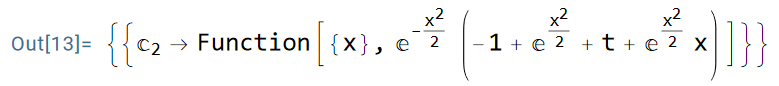
\includegraphics[scale=0.5]{img6}
$$
Подставляем найденные $C_1(y)$ и $C_2(x)$ в полученное ранее решение. Тогда
\begin{listingcont}
In[18]:= u[x, y] /. usol /.c1sol[[1]] /. c2sol[[1]]
\end{listingcont}
$$
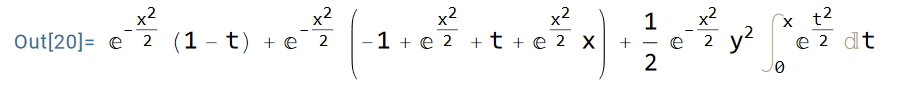
\includegraphics[scale=0.5]{img7}
$$
Для того, чтобы избавиться от введенной постоянной $t$, упростим выражение:
\begin{listingcont}
In[19]:= % // Simplify
\end{listingcont}
$$
	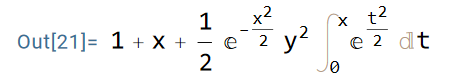
\includegraphics[scale=0.5]{img8}
$$
В итоге получили решение исходной задачи Гурса $$u(x,y) = 1+x+\dfrac{y^2}{2}e^{-\frac{x^2}{2}}\int\limits_0^x e^{\frac{\xi^2}{2}}d\xi.$$
С помощью подстановки в поставленную задачу убедимся в том, что мы действительно нашли верное решение:
$$
	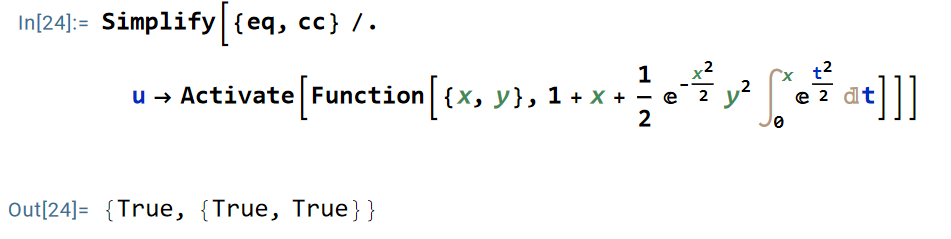
\includegraphics[scale=0.5]{img9}
$$
То есть построенное частное решение удовлетворяет поставленной задаче.\\\\
Графически изобразим полученную поверхность. К примеру, возьмем область $[-2, 4]\times [-4, 2]$. Тогда
$$
	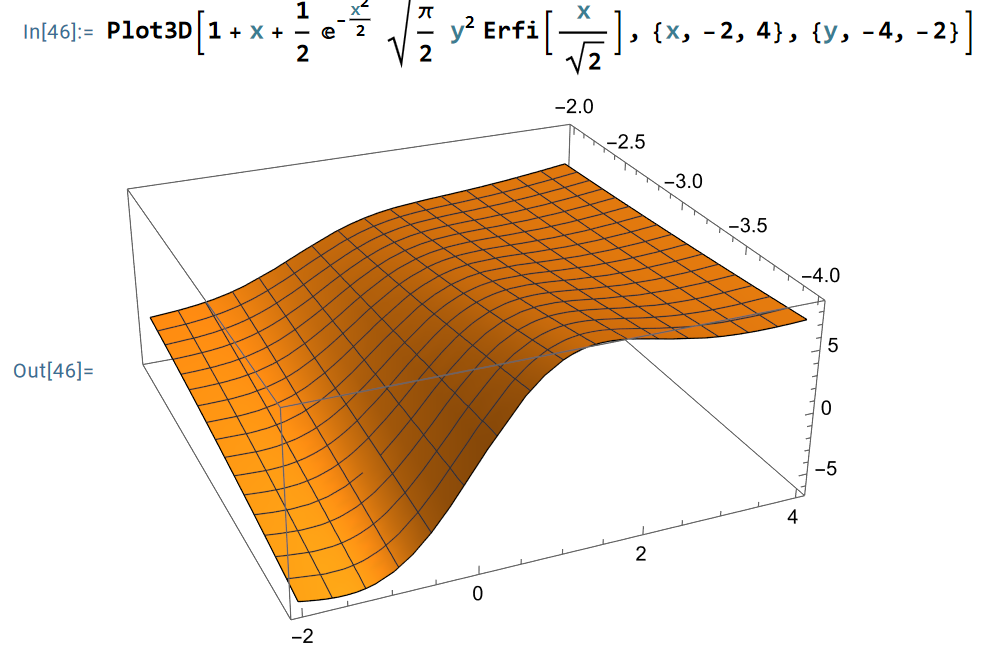
\includegraphics[scale=0.5]{img10}
$$
\section*{Вывод.}
Таким образом, мы нашли решение поставленной задачи Гурса с помощью пакета Wolfram Mathematica, применяя также аналитические рассуждения. Проверили путем подстановки, является ли полученная функция решением поставленной задачи и изобразили графически поверхность, которую задает построенная нами функция. Подобным образом можно решать и другие задачи, поставленные для дифференциальных уравнений в частных производных.
\end{document}

 